\label{fundamentacao_teorica}

%%%%%%%%%%%%%%%%%%%%%%%%%%%%%%%%%%%%%%%%%%%%%%%%%%%%%%%%%%%%%%%%%%%%%%%%%%%%%%%

\newcommand{\texCommand}[1]{\texttt{\textbackslash{#1}}}%

\newcommand{\exemplo}[1]{%
\vspace{\baselineskip}%
\noindent\fbox{\begin{minipage}{\textwidth}#1\end{minipage}}%
\\\vspace{\baselineskip}}%

\newcommand{\exemploVerbatim}[1]{%
\vspace{\baselineskip}%
\noindent\fbox{\begin{minipage}{\textwidth}%
#1\end{minipage}}%
\\\vspace{\baselineskip}}%

%%%%%%%%%%%%%%%%%%%%%%%%%%%%%%%%%%%%%%%%%%%%%%%%%%%%%%%%%%%%%%%%%%%%%%%%%%%%%%%

Este capítulo descreve a revisão conceitual sobre as tecnologias relacionadas ao tema deste projeto. 

%%%%%%%%%%%%%%%%%%%%%%%%%%%%%%%%%%%%%%%%%%%%%%%%%%%%%%%%%%%%%%%%%%%%%%%%%%%%%%%%

\section{Monitoramento de Sistemas Distribuídos}%

O monitoramento é forma utilizada para acompanhar ou observar o andamento de um fluxo ou processo, na área de tecnologia da informação é responsável por verificar e coletar informações sobre funcionamento de ativos de rede ou serviços, com propósito de apresentar informações mais resumidas e favoráveis em painéis ou sistemas para a realização de monitoramento\cite{de2014indicadores}. O monitoramento é necessário para uma série de fins, incluindo a verificação de status, solução de problemas, ajustes de desempenho e depuração\cite{hollingsworth2003instrumentation}. 

A intenção de monitorar ativos de rede e serviços, é mante-los sempre disponíveis, seja pelo mau funcionamento de um ativo de rede, serviço ou por uma indisponibilidade(queda de energia ou internet). Como mencionado anteriormente o ato de acompanhar o funcionamento desses recursos propõem ao gestores desse processos encontrar uma forma mais visível e gerenciável para solucionar problemas, alertar sobre possíveis falhas ou até determinar uma situação para o retorno automático desses serviços. 

O CPD, atualmente possui um serviço que executa o monitoramento em tempo de execução, porém a forma utilizada para o monitoramento foi a leitura do arquivo de \textit{log}, pois havia um grande preocupação com \textit{trade-off} gerado. A fim de obter melhor custo de monitoramento x desempenho tomou-se a decisão pela coleta das informações de monitoramento por meio dos \textit{logs} gerados pelo ErlangMS \cite{filgueirasmonitoramento}.    

O monitoramento implantado no \acrshort{CPD} para acompanhamento dos sistemas e serviços(\textit{web services}), desenvolvidos pela unidade de desenvolvimento \textit{software} utilizando o Barramentos de serviços ErlangMS, não possui um acompanhamento especifico no funcionamento dos seus serviços, visto que há casos e relatos de usuários que acessam os sistemas, realizam a autenticação, clicam nos menus, mas nada aparece como resultado das pesquisas e funcionalidades dos sistemas. Por dispor de uma arquitetura orientada a serviços a camada de apresentação funciona normalmente, mas os recursos(\textit{web services}) encontram-se indisponíveis.

Sistemas distribuídos podem ser interpretados como aplicações distintas que possuem um \textit{middleware} que realize algum tipo de conexão entre as aplicações \cite{penteado2012jmonitor}. Esses sistemas ou aplicações podem funcionar com seus serviços de forma independente, ou dependente de outros serviços de aplicações distintas, o funcionamento desses serviços são essenciais, principalmente os que são dependentes, por esse motivo a implantação do monitoramento de sistemas distribuídos é utilizada para um melhor acompanhamento e gerenciamento das aplicações e serviços para verificar o funcionamento e disponibilidade.   

%%%%%%%%%%%%%%%%%%%%%%%%%%%%%%%%%%%%%%%%%%%%%%%%%%%%%%%%%%%%%%%%%%%%%%%%%%%%%%%%

\section{Arquitetura Orientada a Serviços - SOA}

A Arquitetura Orientada a Serviços pode ser descrita com um estilo arquitetural capaz de realizar a comunicação entre aplicações heterogêneas por meio de mensagens\cite{fraser2007service}. É comum que essas aplicações possuam estruturas e linguagens completamente distintas, pois as aplicações envolvidas, normalmente independem umas das outras e precisam que essa comunicação aconteça, mas para que haja a comunicação interoperável entre as aplicações é previsto na arquitetura \acrshort{SOA} que a as funcionalidade possam ser disponibilizadas por meio de serviços(\textit{web services}) em componentes distribuídos, que ao mesmo tempo que possam fornece-los possam também consumi-los\cite{sward2011service,bianco2011architecting}.

Com o aumento da utilização da arquitetura percebeu-se a necessidade de discussões e definições afim abraçar os conceitos da arquitetura \acrshort{SOA}, com as discussões decidiu-se não apenas criar conceitos, mas também orientações  afim  de guiar as organizações de maneira consistente e sustentável, de modo a agregar valor ao negócio, com maior agilidade e efetividade de custos, em alinhamento com a dinâmica das necessidades de negócio, e foi a partir desse movimento que surgiu o Manifesto \acrshort{SOA} \cite{erl2009soa} priorizando os seguintes itens:

\begin{itemize}

\item Valor do negócio em relação a estratégia técnica;

\item Objetivos estratégicos em relação a benefícios específicos de projetos;

\item Interoperabilidade intrínseca em relação a integração personalizada;

\item Serviços compartilhados em relação a implementações de propósito específico;

\item Flexibilidade em relação a otimização; e

\item Refinamento evolutivo em relação a busca da perfeição inicial.

\end{itemize}

Para realização da comunicação entre as aplicações ou serviços em componentes distribuídos no estilo arquitetural \acrshort{SOA}, \cite{clements2002documenting} descreve em seu trabalho que a comunicação poderá ser executada por meio de um intermediador ou na falta dele poderá ser realizada ponto-a-ponto, entre os intermediadores o estilo arquitetural \acrshort{SOA} dispõe dos seguintes tipos de componentes que compõem uma arquitetura orientada a serviços, são eles \cite{bass2003software}:

\begin{itemize}

\item Prestador de serviços;

\item Consumidores de serviço;

\item \acrfull{ESB};

\item Registro de serviços;

\item \textit{Server Orchestration}; 

\item \acrfull{SOAP}.

\item \acrfull{REST}

\item Conector de mensagens assíncronas

\end{itemize}

Com a utilização desses componentes \cite{bass2003software} trata como principal benefício de uma arquitetura \acrshort{SOA} a interoperabilidade, pois permite que aplicações, dispositivos, sistemas e serviços heterogêneos possam realizar a comunicação entre si, fornecendo e consumindo informações  de forma integrada. 

O \acrshort{CPD} para implementação e implantação da arquitetura \acrshort{SOA} na modernização dos seus sistemas, escolheu como componente o \acrshort{ESB} e como plataforma o barramento ErlangMS\cite{Agilar},que atua como intermediador prestando serviço de mensageria.

%%%%%%%%%%%%%%%%%%%%%%%%%%%%%%%%%%%%%%%%%%%%%%%%%%%%%%%%%%%%%%%%%%%%%%%%%%%%%%%%

\section{ESB}

Um componente \acrshort{ESB} é responsável por fornecer serviço de infraestrutura e mediar a comunicação por meio de serviços entre aplicações consumidoras e fornecedoras de serviços, fazendo de forma uniforme a transmissão das mensagens por meio de um protocolo ou tecnologia, utilizando conectores do tipo \textit{Call-return}, onde os mais comuns e também mais utilizados no mercado são o \acrshort{SOAP} e o \acrshort{REST}  	 \cite{clements2002documenting}.

Para a implementação de um \acrshort{ESB} no estilo \acrshort{SOA} devem ser seguidos alguns itens primordiais para o funcionamento, mas primeiro a organização ou instituição deverá avaliar as tecnologias utilizadas em seus sistemas ou serviços, visto que, a complexidade de uma arquitetura \acrshort{SOA} é alta, e dependendo da situação não é necessário a implementação ou implantação de um \acrshort{ESB} quando por exemplo, uma organização que  possui em sua arquitetura de sistemas a mesma linguagem, plataforma e tecnologia, podendo fazer a comunicação ou troca de mensagens ponto-a-ponto\cite{bianco2011architecting}. No caso em que existe a necessidade da implementação ou implantação de um \acrshort{ESB}, a padronização e táticas descritas em \cite{bianco2011architecting} que devem ser seguidas, e de acordo com \cite{erl2009soa} possuem as seguintes características, são elas:

\begin{itemize}

\item Roteamento Intermediário: Um serviço de roteamento genérico intercepta mensagens e com base no encaminhamento a lógica que determina para onde as mensagens devem ser enviadas.

\begin{itemize}

\item Balanceamento de carga: Possuir um \textit{Failover} para um \textit{backup} no caso de o serviço de destino 	primário não estar disponível.

\item{Seleção da versão do Serviço: Verificar se os pedidos são enviados para versões compatíveis de um serviço para     suportar compatibilidade com versões anteriores durante os períodos de transição}.

\item Serviço de seleção com base em dados da mensagem: Verificar se pedidos de clientes são enviados para um componente de processamento mais rápido.

\item Regras de controle de acesso: Analisar um pedido de um usuário não autenticado é encaminhado para um início de sessão página.

\item Tratamento de exceções: Apresentar uma mensagem de erro de resposta que é redirecionada para um serviço responsável para manipulação de exceção centralizada.

\end{itemize}

\item O \textit{Service Broker}: Integrar componentes que foram desenvolvidos em diferentes linguagem por diferentes organizações.

\begin{itemize}

\item Modelo de Transformação de Dados: Os dados enviados do consumidor de serviços numa dada estrutura transforma-se em uma estrutura diferente, que está prevista para o prestador de serviços.

\item Conversão de Formato de dados: Usar sempre consumidor de serviço e o fornecedor precisa de trocar dados representados em diferentes formatos como por exemplo, \acrshort{XML}, \acrshort{CSV}, \acrshort{JSON}.

\item Protocolo \textit{Bridging}: O consumidor de serviço envia uma solicitação usando um protocolo e o \textit{Service Broker} intercepta o pedido e o converte para um pedido ao fornecedor do serviço usando um protocolo diferente.

\end{itemize}

\item Mensagens \textit{Asynchronous}: Alguns \acrshort{ESB}s fornecem capacidade suficiente para que o sistema de mensagens permita que os pedidos e respostas de um serviço possam ser trocados através de canais de mensagens.

\item Interceptor: Alguns \acrshort{ESB}s oferecem a capacidade de configurar interceptores, que são elementos de software que são ativados para todas as solicitações e respostas.

\end{itemize}

O \acrshort{ESB} a ser implementado deve possuir vantagens e benefícios que uma arquitetura \acrshort{SOA} pode fornecer, para alcança-los \cite{bianco2011architecting} cita os seguintes itens(Atributos de Qualidade), como representação de um \acrshort{ESB} padronizado e operável, o atendimento à esses itens são de suma importância, são eles:

\begin{itemize}

\item Interoperabilidade: O \acrshort{ESB} permite que sistemas diferentes possam interoperar, por meio de protocolos de comunicação e tecnologias de implementação. 

\item Modificabilidade: A capacidade de executar a transformação do modelo de dados que permite a implantação de novas versões de um serviço sem interromper consumidores de serviços existentes. 

\item Confiabilidade: Quando o receptor de uma solicitação de serviço ou resposta falhou, e o ESB cria ou gera uma fila para que mensagem seja executa quando o serviço estiver disponível novamente. 

\item Segurança: O \acrshort{ESB} pode incluir a funcionalidade de controle de acesso. Pode aplicar a autenticação e regras de autorização em trocas de mensagens de serviço.

\end{itemize}

Como desafio o \acrshort{ESB} deve responder a altura seus \textit{trade-offs},  principalmente em uma arquitetura complexa como essa, entre os desafios que deverão ser suportados, para um bom funcionamento da plataforma, \cite{bianco2011architecting} cita a:

\begin{itemize}

\item Manutenibilidade: Ter cuidado e atenção ao especificar demais a codificação do ESB, ao ponto de restringir comunicação com outras tecnologias. 
 	
\item Performance: Não permitir a perda comprometedora no desempenho do \acrshort{ESB} por conta das logicas de roteamento ou interpretação dos dados durante a comunicação.

\item Segurança: verificar a configuração a fim de evitar acessos não autorizados ao \acrshort{ESB}.

\item Disponibilidade: O \acrshort{ESB} pode ser um ponto único de falha no sistema.

\end{itemize}

%%%%%%%%%%%%%%%%%%%%%%%%%%%%%%%%%%%%%%%%%%%%%%%%%%%%%%%%%%%%%%%%%%%%%%%%%%%%%%%%

\section{REST}

A Transferência de Estado Representacional - \acrshort{REST} pode ser definida como um estilo arquitetural hibrido derivado de vários dos estilos arquiteturais baseados em rede e que define um conjunto de restrições e propriedades baseados no protocolo de comunicação \acrshort{HTTP}, com a intenção de fornecer a interoperabilidade entre sistemas, serviços e aplicações distribuídas conectadas a rede mundial de computadores - \acrshort{WWW} para a realização de troca de informações \cite{fielding2000architectural}. Os \textit{web services} compatíveis com \acrshort{REST} permitem que os sistemas solicitantes acessem e manipulem representações textuais de recursos da \textit{Web} utilizando um conjunto uniforme e predefinido de operações sem estado. O estilo arquitetural proposto por Roy Fielding que inspirou a criação do documento de arquitetura definido pelo \acrshort{TAG} - \acrshort{W3C},  quanto muitos outros arquitetos de \textit{softaware}, que o veem como um modelo norteador para construir e padronizar serviços da Web \cite{booth2013web}. O \acrshort{REST} fornece semântica para uniformizar sua interface, principalmente no que tange a  operações para criar, recuperar, atualizar e excluir dados, e  também a possibilidade da utilização de padrões de tecnologia como \acrshort{XML} e o \acrshort{JSON}. 

Em \acrshort{REST} as principais operações por meio do protocolo \acrshort{HTTP} são:

\begin{itemize}

\item POST: Cria uma nova entidade ou recurso. 

\item GET: Recupera a informação de um recurso.

\item PUT: Atualiza os dados de um recurso informado.

\item DELETE: Exclui os dados de um recurso informado.

\end{itemize}

%%%%%%%%%%%%%%%%%%%%%%%%%%%%%%%%%%%%%%%%%%%%%%%%%%%%%%%%%%%%%%%%%%%%%%%%%%%%%%%%

\section{JSON}

\acrfull{JSON} é um formato baseado em texto, de fácil leitura e interpretação para humanos, para a leitura de máquinas o \acrshort{JSON} é baseado em um subconjunto da linguagem de programação \textit{JavaScript}, e por possuir um um padrão, seu funcionamento independe de uma tecnologia ou linguagem de programação, focando princialmente na troca de dados e mensagens \cite{bray2017javascript}.

Por decisão técnica especificamente relacionada a interoperabilidade e o baixo acoplamento o barramento utilizado pelo \acrshort{CPD} o Erlangms, utiliza o \acrshort{JSON} por conta do  baixo\textit{overhead} gerado na troca de mensagens em relação as trocas de mensagens feitas com a utilização protocolo \acrshort{SOAP} com a linguagem \acrshort{WSDL}, e apontando também o nível baixa da curva de aprendizagem para a utilização do \acrshort{JSON}.

%%%%%%%%%%%%%%%%%%%%%%%%%%%%%%%%%%%%%%%%%%%%%%%%%%%%%%%%%%%%%%%%%%%%%%%%%%%%%%%%

\section{ErlangMs}
O Barramento de serviços da \acrshort{UnB} denominado Erlangms foi conceituado em uma disciplina do \acrshort{MPCA} e proposto como trabalho para solucionar alguns problemas relacionados a quantidade de sistemas heterogêneos, defasagem tecnológica das aplicações e a falta de um padrão de comunicação entre eles no \acrshort{CPD} \cite{Agilar}. 

O Erlangms dispõem de uma arquitetura \acrshort{SOA} utilizando o estilo arquitetural \acrshort{REST} e sua implementação foi feita na linguagem funcional Erlang. O barramento atualmente está implantado no \acrshort{CPD} e  funcionando com um serviço de mensageria. A realização da comunicação e troca de mensagens dos sistemas e clientes é feita por meio de serviços(\textit{web services}) utilizando o formato \acrshort{JSON}. O Erlangms tem sua arquitetura é apresentada na figura \ref{fun:fig:erlangms} .

\begin{figure}[h!]
	\begin{center}
	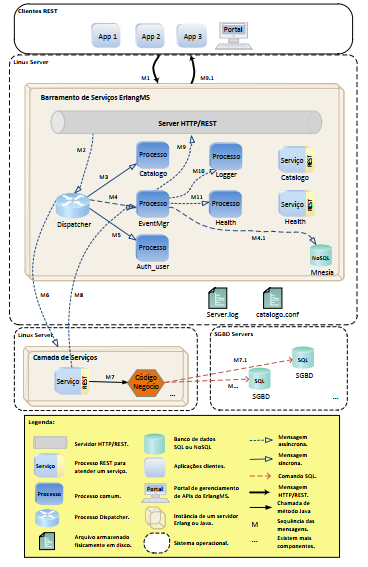
\includegraphics[scale = 1.20]{img/Arquitetura_ErlangMS.png}
		\caption{Arquitetura do trabalho Erlangms descrita por\cite{Agilar}}
		\label{fun:fig:erlangms}
	\end{center}
\end{figure}
%%%%%%%%%%%%%%%%%%%%%%%%%%%%%%%%%%%%%%%%%%%%%%%%%%%%%%%%%%%%%%%%%%%%%%%%%%%%%%%%

\section{Ferramentas de Monitoramento}

\begin{enumerate}
\item Nagios\textsuperscript{\textregistered}

O Nagios\textsuperscript{\textregistered} é uma aplicação com interface \textit{web} para o monitoramento de rede baseada na web idealizada e desenvolvida por Ethan Galstad \cite{bin2011new}. O Nagios\textsuperscript{\textregistered} é projetado para a realizar o acompanhamento de ativos de rede, sistemas e serviços com a finalidade de notificar os usuários e responsáveis pelos ativos de rede, sistema e serviços que estão registrados na ferramenta como contatos emergências, em caso aconteça alguma anomalia ou problema durante o funcionamento da rede, sistemas e serviços.

O Nagios\textsuperscript{\textregistered} é tratado como uma ferramenta que possui um alta complexidade em sua configuração, pois possui uma gama de recursos e funcionalidades disponíveis para a utilização, devido a grande quantidade de recursos o Nagios\textsuperscript{\textregistered} é bastante utilizado ele também possui um grande número de \textit{plug-ins} disponíveis na para a realização do monitoramento podendo personalizar o monitoramento de serviços como SMTP, POP3, HTTP, PING \cite{lcc2012nagios}. Nesse projeto o Nagios\textsuperscript{\textregistered} será utilizado com ferramenta de monitoramento dos sistemas e serviços fornecidos pela \acrshort{UnB} com utilização de serviço SMTP para o monitoramento, visto que, o \acrshort{CPD} já utiliza a ferramenta para o monitoramento dos ativos de rede de toda a universidade. 

\begin{figure}[h!]
	\begin{center}
	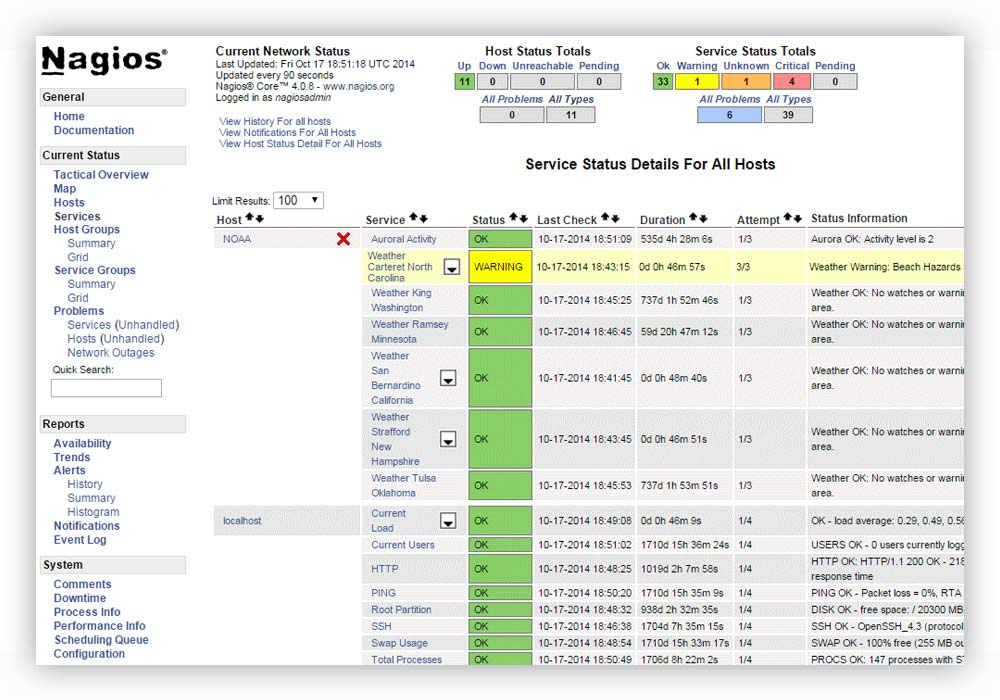
\includegraphics[scale = 0.39]{img/Comprehensive_Monitoring_Drop2.jpg}
		\caption{Monitoramento de componentes\cite{lcc2012nagios}}
		\label{fun:fig:nagios}
	\end{center}
\end{figure}

\item Ganglia

 O Ganglia é um \textit{software} de monitoramento escalonável com a finalidade de coletar dados para acompanhar o funcionamento de sistemas distribuídos e sistemas de alto desempenho, como \textit{clusters}. Por conta da estrutura hierárquica implementada, o \textit{software} utiliza a linguagem de marcação de texto XML para a representação dos dados. 
 
 O Ganglia é baseado em um protocolo \textit{multicast} de escuta e anuncio, e necessariamente precisa ter em cada \textit{host} que será monitorado a instalação de um \textit{Gmond} \cite{vyas2014embedding}. O \textit{Gmond} é um serviço em execução em cada \textit{host} que coleta as informações de estado de um \textit{host} de forma individual e insere essas informações no canal de comunicação \textit{multicast} para enviar esse dados ao Ganglia.
 
 \begin{figure}[h!]
	\begin{center}
	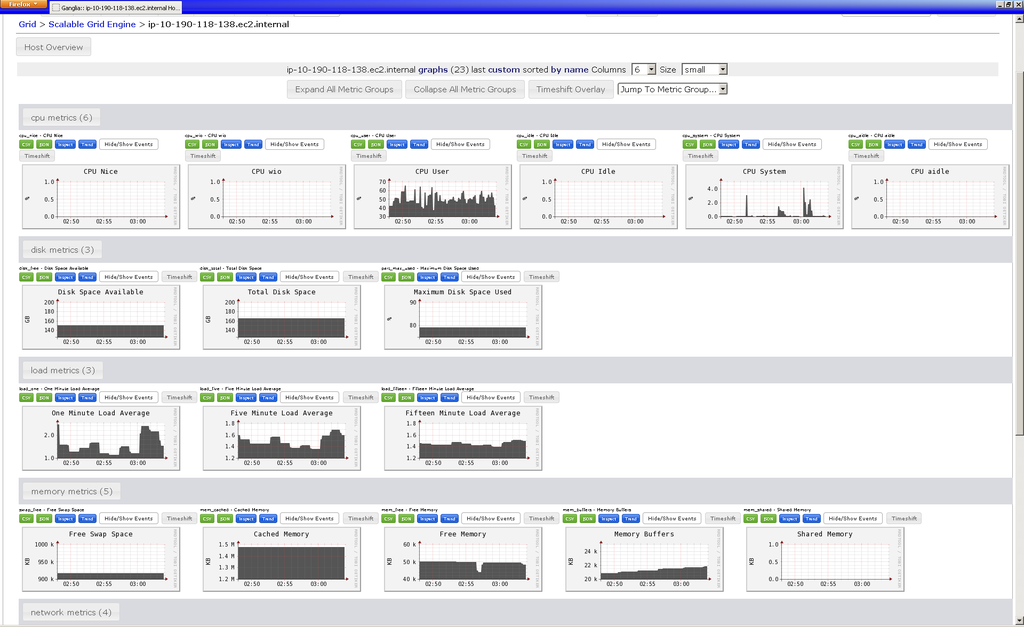
\includegraphics[scale = 0.50]{img/1024px-ScalableGridEngineGanglia2.png}
		\caption{Monitoramento de \textit{clusters} \cite{Ganglia}}
		\label{fun:fig:ganglia}
	\end{center}
\end{figure}
 
 
 Em uma breve análise após a utilização das ferramentas de monitoramento \cite{benincosa2ganglia} cita em seu artigo os seguintes itens:
\begin{itemize}

\item O Ganglia não possui um sistema de notificação integrado enquanto que o Nagios\textsuperscript{\textregistered} se destaca nisso.
\item Já o Nagios\textsuperscript{\textregistered} não possui agentes integrados escaláveis nos \textit{hosts} de destino (um motivo de reclamação das pessoas), enquanto que isso já faz parte do projeto original e intencional do Ganglia.

\end{itemize}

 Diante desse cenário a autora sugere a utilização das ferramentas em conjunto de modo que sejam utilizados em sua potencialidade, porém como \acrshort{CPD} já utiliza o Nagios\textsuperscript{\textregistered} e a intenção da Gestão \acrshort{CPD} e do projeto é trabalhar com o acompanhamento a notificação dos serviços caso haja alguma falha ou mau funcionamento, como o Ganglia não executa uma das principais funcionalidades do monitoramento, a ferramenta não entrará como \textit{software} a ser utilizado no projeto.
 
\item Cacti

O Cacti é uma ferramenta de monitoramento que coleta e analisa informações por meio de gráficos em tempo de execução, com um excelente desempenho, o monitoramento pode ser feito em redes complexas e ativos de rede. O Cacti armazena suas informações coletadas em bancos de dados, para para coleta das informações são necessários \textit{scripts}/comandos que são implementados em cada ativo e são denominados cactos, e para a apresentação dos gráficos é necessária a utilização do \textit{software}  \acrfull{RRDTool} que possui uma apresentação gráfica bastante intuitiva e de fácil utilização \cite{cacti}.

O \acrshort{RRDTool} é uma ferramenta que realiza o registro de dados e gráficos de alto desempenho para dados de séries temporais, e como os cactos implementados nos \textit{hosts} são \textit{scripts} o \acrshort{RRDTool} pode ser facilmente integrado com  \textit{scripts} de \textit{shell} \cite{rrdtool}. 

\begin{figure}[h!]
	\begin{center}
	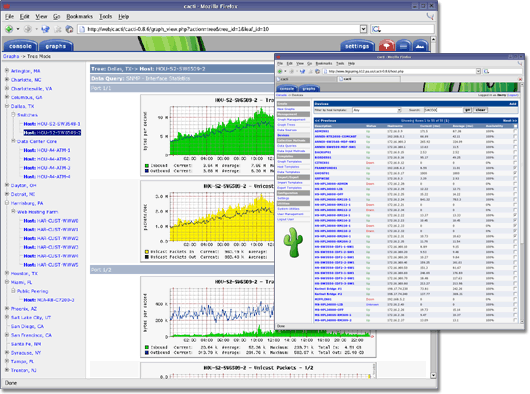
\includegraphics[scale = 0.50]{img/cacti_promo_main.png}
		\caption{Monitoramento de rede \cite{cacti}}
		\label{fun:fig:cacti}
	\end{center}
\end{figure}

O Cacti possui \textit{plugins} para integração com outras funcionalidades e ferramentas, incluído o protocolo \acrshort{SNMP}, mas não é o seu foco devido a preocupação com o desempenho na troca de informações e no monitoramento. Como o trabalho visa uniformizar o meio de comunicação entre as aplicações e definir especificamente o protocolo \acrshort{SNMP} para transmitir informações para a realização do monitoramento, esse \textit{software} não será utilizado no projeto.

\begin{figure}[h!]
	\begin{center}
	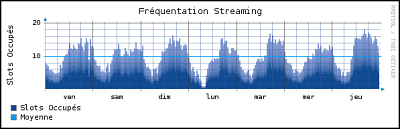
\includegraphics[scale = 0.50]{img/stream-pop.png}
		\caption{Gráfico de monitoramento do RRDTool \cite{rrdtool}}
		\label{fun:fig:rrdtool}
	\end{center}
\end{figure}

\item Zabbix

O Zabbix é uma solução tecnológica conceituada e desenvolvida para a realização de monitoramento de rede, servidores e serviço. O monitoramentos poderá ser realizado com o agrupamento desses recursos objetivando potencialização das vantagens de utilização dos ativos de TI ou diminuição os riscos da utilização desses ativos aos usuários, esse procedimento é denominado \textit{pooling} ou por mensagens de notificações e alertas por meio de \textit{trapping} \cite{contessa2010gerenciamento}. O Zabbix tem como idealizador  Alexei Vladishev, e atualmente é mantido pela Zabbix SIA \cite{zabbix}.   

Como as demais aplicações e \textit{softwares} citados anteriormente o Zabbix possui funcionalidades para o monitoramento que realizam a coleta de dados por servidor ou agentes, a ferramenta tem suporte ao protocolo \acrshort{SNMP} e também interface \textit{web} para visualização de gráficos gerados por meio dos dados coletados dos \textit{hosts} ou agentes. Por definição arquitetural o Zabbix é composto por componentes com funcionalidades primordiais para o seu funcionamento são eles \cite{zabbix}: 

\begin{itemize}
\item Servidor Zabbix;
    \begin{itemize}
        \item é o componente central do Zabbix; realiza o monitoramento, interage com os proxies e agentes, calcula as mudanças de estado nas \textit{triggers}, envia notificações, controla o repositório central de dados.
    \end{itemize}
\item Agente Zabbix;
\begin{itemize}
        \item é o componente instalado nos servidores monitorados, usado para monitorar ativamente seus recursos e aplicações.
    \end{itemize}
\item Proxy Zabbix;
\begin{itemize}
        \item é o componente com capacidade de realizar a coleta de dados no lugar do Servidor Zabbix, distribuindo a carga de processamento.
    \end{itemize}
\end{itemize}

Em comparação com as ferramentas de monitoramento mais utilizadas atualmente, \cite{marik2014comparative} descreve em seu artigo que o Zabbix está entre as melhores aplicações, incluído as citadas nesse trabalho, por possuir pré-requisitos básicos na instalação e configuração, excelente tempo de resposta em caso de falhas de serviços e de recursos de \acrshort{TI} e as notificações por e-mail e \acrshort{SMS}, porém o \textit{dashboard} para a realização do monitoramento é complexo e não intuitivo ao usuário, como pode ser visualizado a seguir na figura \ref{fun:fig:zabbix}, podendo não auxiliar em um gerenciamento adequado aos serviços e aplicações que são monitoradas, apesar de uma boa aplicação de monitoramento, o Zabbix não será utilizado com ferramenta de monitoramento para esse trabalho.    

\begin{figure}[h!]
	\begin{center}
	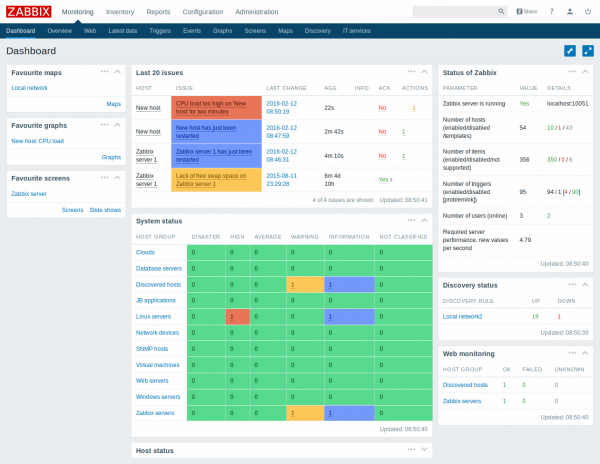
\includegraphics[scale = 0.80]{img/dashboard.png}
		\caption{\textit{Dashboard} de monitoramento \cite{zabbix}.}
		\label{fun:fig:zabbix}
	\end{center}
\end{figure}

\end{enumerate}

%%%%%%%%%%%%%%%%%%%%%%%%%%%%%%%%%%%%%%%%%%%%%%%%%%%%%%%%%%%%%%%%%%%%%%%%%%%%%%%%

\section{Agentes de Monitoramento}

Em uma arquitetura de monitoramento de serviços ou ativos de rede que utiliza o protocolo \acrshort{SNMP}, é necessária a implementação de agentes de monitoramento para a instalação em \textit{hosts} e dispositivos que serão monitorados, esse agentes consistem em coletar dados e enviar mensagens de alerta ao gerentes de monitoramento, como  apresentado na figura \ref{fun:fig:agente}, como por exemplo, o uso de \acrshort{CPU} e a quantidade de memória de utilização de um processo ou um alerta de falha de um dispositivo ou serviço \cite{7439952}.  

\begin{figure}[h!]
	\begin{center}
	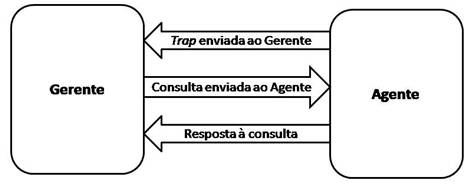
\includegraphics[scale = 0.80]{img/image004.jpg}
		\caption{Esquema de comunicação entre os agentes e as estações de gerenciamento \cite{snmpagentimage}.}
		\label{fun:fig:agente}
	\end{center}
\end{figure}

Um agente de monitoramento pode ser definido como um componente ou aplicação de gerenciamento de rede ou serviço no dispositivo a ser gerenciado e possuem duas operações básicas \textit{GET} e \textit{SET}, o agente em execução fica responsável por exportar os dados de gerenciamento dos sistemas, serviços ou ativos de rede gerenciados com variáveis organizadas de forma hierárquica. Essa hierarquia é contemplada por metadados que são representados por \acrshort{MIBs}, e \acrshort{MIBs} por sua vez são um conjunto dos objetos gerenciados, que procuram abranger todas as informações necessárias para a gerência de rede \cite{6240708}. Nesse trabalho o agente de monitoramento utilizado é o Exometer que funciona como agente de monitoramento responsável pela coleta das informações geradas pelo Barramento de serviços Erlangms e a transmissão dessas informações ao Nagios\textsuperscript{\textregistered} por meio do protocolo \acrshort{SNMP}. 

%%%%%%%%%%%%%%%%%%%%%%%%%%%%%%%%%%%%%%%%%%%%%%%%%%%%%%%%%%%%%%%%%%%%%%%%%%%%%%%%

\subsection{Exometer}

\begin{figure}[h!]
	\begin{center}
	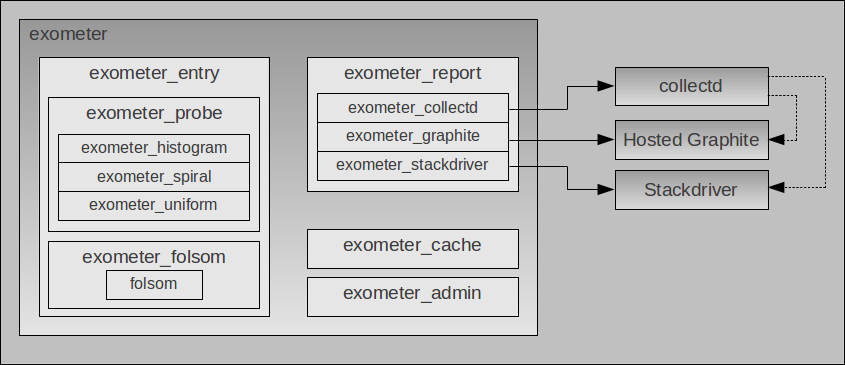
\includegraphics[scale = 0.60]{img/exometer_overview.png}
		\caption{Arquitetura do Exometer \cite{exometer_core}.}
		\label{fun:fig:zabbix}
	\end{center}
\end{figure}
O Exometer é um \textit{framework} capaz de executar a instrumentação e permitir a exportação de dados de maneira fácil e eficiente utilizando bibliotecas implementadas em código Erlang, normalmente os dados exportados são relacionados ao desempenho dos sistemas e serviços. Com a utilização de módulos, o Exometer pode realizar a integração com uma grande variedade de sistemas de monitoramento, nesse trabalho a integração é com a aplicação de monitoramento Nagios\textsuperscript{\textregistered}. O potencial do Exometer é fornecer métricas de várias formas e parâmetros, para isso dispõem de um conjunto de componentes para monitoramento pré-definidos e que podem ser estendidos de forma personalizada para lidar com diversos tipos de métricas e alguns protocolos \cite{exometer_core}.




%%%%%%%%%%%%%%%%%%%%%%%%%%%%%%%%%%%%%%%%%%%%%%%%%%%%%%%%%%%%%%%%%%%%%%%%%%%%%%%%

\section{Métricas de Monitoramento}

A métrica de \textit{software} vem representando um papel importante para o funcionamento adequado das aplicações \cite{de2016metrica}. À medida que os sistemas e serviços crescem em quantidade, tamanho, complexidade e criticidade, a necessidade de monitorá-los é cada vez mais evidente. O monitoramento representa o acompanhamento dessas aplicações de forma detalhada e clara aos responsáveis pela as aplicações \cite{5298441}. A ISO/IEC 9126-1 \cite{associaccao2003nbr} descreve e normatiza a forma para medir a qualidade de \textit{software}, de acordo com a norma \cite{associaccao2003nbr}, a métrica é o método e escala de medição definidos, a métrica pode ser direta ou indireta, a medição de uma métrica direta se dá quando não depende de medidas de outros atributos e a métrica indireta se dá quando há ou existe a necessidade de derivação de um ou mais atributos de medição.
No que tange um ambiente computacional, as métricas ajudam a medir o \textit{software} de um forma eficaz, para isso é preciso que as métricas sejam bem definidas, justificadas e formalizadas, além disso é desejável que as métricas apresentem de forma clara o que está sendo medido, descrevam rapidamente a medição sem custeio computacional alto e que o resultado do que está sendo medido não seja mudado ou sofra interferência em seu resultado caso haja a mudança de \textit{software}, plataforma ou linguagem de programação\cite{meirelles2013monitoramento}.


%%%%%%%%%%%%%%%%%%%%%%%%%%%%%%%%%%%%%%%%%%%%%%%%%%%%%%%%%%%%%%%%%%%%%%%%%%%%%%%%


\section{Instrumentação}
\label{instrumentacao}
A instrumentação é a ciência que aplica e desenvolve técnicas para adequação de instrumentos para a medição e monitoração. A instrumentação é muito utilizada no ambiente industrial, principalmente no que tange a medição dos equipamentos de produção que necessitam de acompanhamento para verificação de pressão, temperatura, vazão e nível.\cite{ribeiro1999instrumentaccao}. O barramento de serviços ErlangMs dispõem em sua arquitetura uma estrutura definida de fácil implementação para a instrumentação, possui um modelo de dados em que são registrados contadores. No modelo de dados são registradas algumas informações como a data e hora do registro, o identificador do contador e o contador.  
Segundo \cite{frota2008educaccao} a instrumentação pode ser utilizada como um componente de processamento da informação de sistemas de medição. Por isso a instrumentação pode ser considerada não apenas como ferramenta de contagem de valores para medição, poderá ser utilizada também como uma forma de aprendizagem e conceitual e científica.  

%%%%%%%%%%%%%%%%%%%%%%%%%%%%%%%%%%%%%%%%%%%%%%%%%%%%%%%%%%%%%%%%%%%%%%%%%%%%%%%%

\section{Protocolos de Monitoramento}

\subsection{SNMP}

O Protocolo Simples de Gerenciamento de Rede (\textit{\acrlong{SNMP}}) é um protocolo da camada de aplicação responsável pela transmissão de dados e informações de gerenciamento e monitoramento entre dispositivos e ativos de rede. O \acrshort{SNMP} é um dos protocolos mais utilizados atualmente, devido a sua arquitetura que dispõe de uma estrutura simples capaz de realizar o monitoramento em tempo real sem comprometer a eficiência que está sendo monitorado\cite{roohi2014application}. Em seu paradigma o \acrshort{SNMP} gerencia os ativos de rede baseando-se no esquema cliente-servidor, onde os dispositivo e ativos de rede recebem um agente para que essas informações sejam coletadas e transmitidas, por conta desse paradigma e fácil implantação a popularidade do protocolo aumentou, permitindo as empresas fornecerem diversos tipos de estruturas denominadas \acrshort{MIBs}. Os \acrshort{MIBs} são objetos criados e definidos por meio de uma estrutura virtual capaz de armazenar de informações de gerenciamento\cite{roohi2014application,presuhn2002management}.

O \acrshort{SNMP} é formado por três componentes \cite{nadeau2003mpls}:  

    \begin{itemize}
    \item \acrshort{SMI}
    
    Que é a linguagem de modelagem dos dados usado para definir \textit{syntax} dos dados de gerenciamento, como por exemplo, o Tipo de objeto "INTEGER".
    
    \item \acrshort{MIBs}
    
    Estrutura usada para formar um modelo de dados do sistema(objetos), responsável por representar o tipo, definir o comportamento e a política de acesso aos objetos.
    
    \item \acrshort{SNMP}
    Que consiste em sua arquitetura, o gerente, um dispositivo a ser gerenciado e um agente, que dispões das seguintes operações:
    
        \begin{itemize}
        \item GET
        
        Operação utilizada para recuperar o valor de uma instância específica de um objeto gerenciado.
        
        \item GET-NEXT
        
        Operação utilizada para percorrer interativamente o \acrshort{OID}.
        
        \item GET-BULK
        
        Operação utilizada para recuperar informações de um grupo de objetos.
        \item SET
        
        Operação utilizada para modificar o valor de uma instancia de objeto.
        \item TRAP
        
        Operação utilizada para que um agente possa reportar uma notificação de forma assíncrona aos gerentes.
        
        \end{itemize}
        
    \end{itemize}
    
Após a realização de uma análise, estudos e definições, obteve-se de forma empírica o respaldo para utilização do protocolo na implementação do projeto, vale também observar que o \acrshort{CPD} utiliza o protocolo para o monitoramento de seus ativos de rede, conforme a representação na figura \ref{fun:fig:snmpexecution} apresentada a seguir.

\begin{figure}[h!]
	\begin{center}
	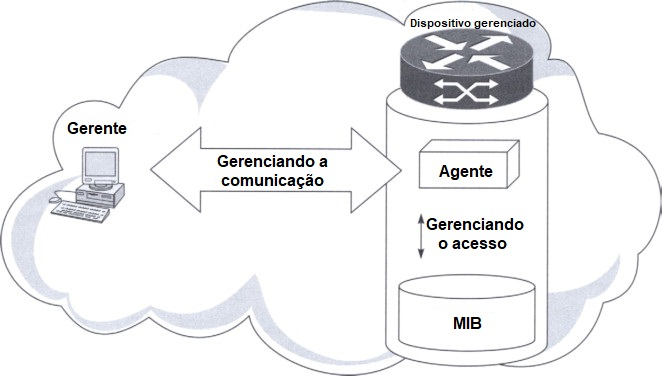
\includegraphics[scale = 0.90]{img/SNMP-Execution.jpg}
		\caption{Gerente e Agente comunicando por meio do protocolo SNMP\cite{nadeau2003mpls}}
		\label{fun:fig:snmpexecution}
	\end{center}
\end{figure}

\subsection{GOSIP}

O \acrshort{GOSIP} é um protocolo pertencente ao modelo \acrshort{OSI} que funciona por meio de software na camada de aplicação em dispositivos \textit{peer-to-peer}, teve seu lançamento anunciado no fim da década de 80 e inicio da década de 90, para facilitar a comunicação e transferência de dados em um modelo governamental prometendo ser a comunicação integrada de sistemas militares do futuro, houve até a formalização de um documento nos padrões \acrshort{RFC} o RFC 1169\cite{mankin1991towards}, porém \cite{harris1992tactical} descreve em seu trabalho que o protocolo proposto foi implementado com seus objetivos bem definidos, mas que não obtiveram o sucesso almejado, pois esperava-se que pela a realização fim-a-fim conseguiriam obter melhores resultados em relação a economia da largura de banda e melhor desempenho com a redundância dos dados.

Apesar dos relatos citados no paragrafo anterior sobre as expectavas não alcançadas com o protocolo, há uma técnica bastante importante que foi extraída, e que é utilizada por meio dos dispositivos de modo a garantir que a comunicação e transmissão da informação sejam garantidas. Diante desse cenário o protocolo trabalha de forma epidêmica, disseminado facilmente as informações nos sistemas distribuídos em larga escala, cujo principal objetivo propagar rapadamente essas informações, o que permite a realização de um monitoramento \textit{peer-to-peer},onde os dispositivo se comunicam diretamente \cite{tanenbaum2007distributed}, a representação dessa propagação poderá ser visualizada na figura \ref{fun:fig:gosip}. 

\begin{figure}[h!]
	\begin{center}
	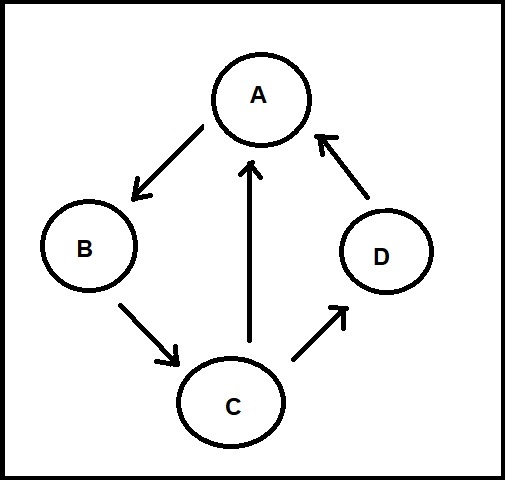
\includegraphics[scale = 0.90]{img/gosip.jpg}
		\caption{Representação de propagação epidêmica \autor{Felipe Evangelista}{dos Santos}  }
		\label{fun:fig:gosip}
	\end{center}
\end{figure}

Nesse trabalho, o \acrshort{GOSIP} não foi utilizado no experimento, foi utilizado como fonte de pesquisa para a realização de um comparativo tecnológico entre os protocolos, que permitiu avaliar e auxiliar na escolha do \acrshort{SNMP} como protocolo ser utilizado no projeto. 

%%%%%%%%%%%%%%%%%%%%%%%%%%%%%%%%%%%%%%%%%%%%%%%%%%%%%%%%%%%%%%%%%%%%%%%%%%%%%%%%

\section{Trabalhos Relacionados}

O autor \cite{abdu1996monitoring} descreve em seu trabalho sobre a opção por investigar a necessidade para realizar o monitoramento de sistemas distribuídos e a necessidade de minimizar a degradação do desempenho do sistemas monitorados. E relatam que a configuração adotada depende da informação a ser monitorada através de diretivas monitoramento.

Seguindo a preocupação com a escalabilidade do monitoramento durante o funcionamento das aplicações \cite{repantis2010scaling} cita sobre a rede Akamai, que permite o processamento de dados de mais de 60.000 servidores de borda em quase em tempo real. A disponibilidade de uma poderosa interface SQL-like para que os dados tem sido um elemento importante na forma como gerimos a nossa rede. Neste trabalho, têm-se centrado sobre as escolhas de design que permitem a consulta para escalar conforme o tamanho da rede, o volume de dados, e o número de consultas crescer. E mostram como consulta aborda esses desafios de escalabilidade, ao fornecer uma latência de dados na ordem de minutos e um tempo médio de resposta de consulta na ordem de décimos de segundo.

O trabalho \cite{subramanyan2000scalable} apresenta estudos sobre o atraso na execução na tarefa de monitoramento devido ao gargalo gerado durante as operações dos agentes,e também descrevem que solução proposta e implementada utiliza o protocolo do monitoramento rede \acrshort{SNMP}, que garante uma facilidade de execução, interoperabilidade e aceitabilidade, e baseia-se nos mais recentes padrões propostas pela RFC 2592.  

Phan \cite{phan2009cryptanalysis} relata em seu trabalho sobre o nível de segurança do protocolo e questiona sobre a falta de confidencialidade e privacidade, itens faltantes no SNMPv1 e, e descreve em seu trabalho  que dispõem de um experimento e recomenda a tulização do SNMPv3.

Com a realização de um análise qualitativa, os autores \cite{lee2004design} buscaram apresentar o funcionamento do protocolo SNMP por meio de experimentos valendo-se de suas vantagens, entre elas seus principais componentes e utilização entre eles: 1) Da estação de gestão; 2) Agente de gestão; 3) Base de informações de gestão; e 4) protocolo de gestão. Eles descrevem o trabalho científico de forma conectada, concisa e objetiva, sobre as técnicas utilizadas para a realização do estudo. O trabalho apresenta uma abordagem orientada a objetos, utilizada para alcançar o projeto sistemático para a implementação de agentes SNMP em sistemas de monitoramento para o gerenciamento remoto.

O artigo \cite{puatruct2010agent} expõe os resultados obtidos no desenvolvimento e manutenção de aplicações distribuídas e sistemas de monitoramento multiagente, com exemplos práticos, a fim de implementar e testar as abordagens teóricas. Os sistemas de monitoramento de agentes múltiplos trazem qualidade e eficiência em quase todas as áreas de atividade, na qual inclui pesquisa científica, educação, saúde ou defesa.
Utilizando os conceitos sólidos da inteligência artificial e reunindo-os para os recursos infinitos dos sistemas distribuídos e da Internet,buscando reduzir a duração do alcance dos objetivos.

Com a leitura e entendimento dos trabalhos pode-se perceber uma preocupação com a utilização do monitoramento em relação ao desempenho, mesmo quando utilizadas técnicas e tecnologias distintas, mas observa-se a importância da realização do monitoramento, visto a grande demanda de \textit{softwares} disseminados na rede mundial de computadores.

%%%%%%%%%%%%%%%%%%%%%%%%%%%%%%%%%%%%%%%%%%%%%%%%%%%%%%%%%%%%%%%%%%%%%%%%%%%%%%%%

\section{Síntese do Capítulo}

Este capítulo apresentou os conceitos e as tecnologias relacionadas ao monitoramento de sistemas distribuídos, \acrshort{SOA}, \acrshort{ESB},  \acrshort{REST}, \acrshort{JSON}, ErlangMs, Ferramentas de Monitoramento, Agentes de monitoramento, Métricas de monitoramento, Instrumentação e Protocolos de monitoramento. As definições e conceitos e tecnologias estudadas foram de grande ajuda tanto para o entendimento do problema quanto para execução e implementação do trabalho. Nesse Capítulo também foram apresentados trabalhos relacionados ao tema tema desse trabalho que colaboraram e orientaram na pesquisa e fundamentação do trabalho. O Capítulo 3 apresenta a realização do mapeamento sistemático.

%%%%%%%%%%%%%%%%%%%%%%%%%%%%%%%%%%%%%%%%%%%%%%%%%%%%%%%%%%%%%%%%%%%%%%%%%%%%%%%%
